\documentclass[12pt]{article}
\usepackage[english]{babel}
\usepackage[utf8x]{inputenc}
\usepackage{amsmath}
\usepackage{graphicx}
\usepackage{float}
\usepackage[colorinlistoftodos]{todonotes}


\setlength {\marginparwidth }{2cm}
\begin{document}

\begin{titlepage}

\newcommand{\HRule}{\rule{\linewidth}{0.5mm}} 

\center 
 

\textsc{\LARGE CUNEF}\\[1.5cm] 
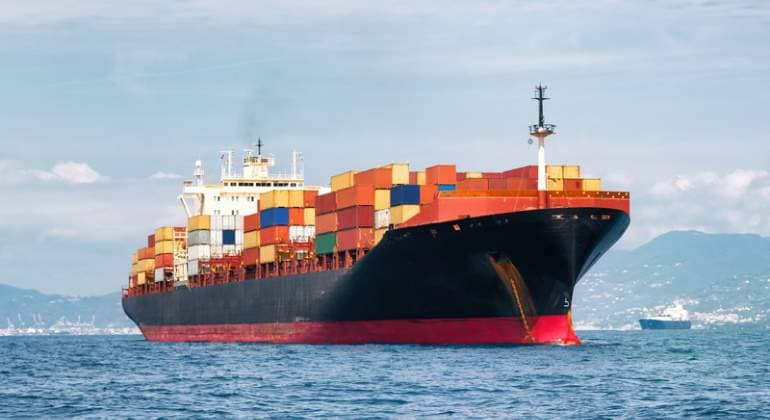
\includegraphics[width=0.5\textwidth]{ALGECIRAS.jpeg}\\[1cm] 
\textsc{\Large Environment Simulation}\\[0.5cm] 

%----------------------------------------------------------------------------------------
%	TITLE SECTION
%----------------------------------------------------------------------------------------

\HRule \\[0.4cm]
{ \huge \bfseries Simulación Puerto}\\[0.4cm] 
\HRule \\[1cm]
 
%----------------------------------------------------------------------------------------
%	AUTHOR SECTION
%----------------------------------------------------------------------------------------

\begin{minipage}{0.4\textwidth}
\begin{flushleft} \large
\begin{center}
\emph{Autores: \\ Jaime Perdiguero Alonso\\ Eduardo Ros Velasco\\ Pablo Martín Tejedor}
 \textsc\\ % Your name
 \end{center}
\end{flushleft}

\end{minipage}\\[1cm]


%----------------------------------------------------------------------------------------
%	DATE SECTION
%----------------------------------------------------------------------------------------

\includegraphics[width=0.2\textwidth]{LOGO CUNEF.png}\\[1cm] 
{\large \today}\\[2cm] 

\vfill 



\end{titlepage}

\begin{center}
   \renewcommand{\contentsname}{Indice de Contenidos}
    \tableofcontents 
\end{center}

\pagebreak


\section{Descripción Idea de Proyecto}
       \subsection{Idea Básica}
        Nuestro concepto de puerto se fundamenta en la optimización de la eficiencia operativa mediante la segmentación de las actividades de carga y descarga en muelles especializados. Hemos diseñado un puerto que se divide en cuatro muelles, cada uno con capacidad para albergar un numero de cargueros simultáneamente (Inicialmente 2). Cada muelle está adaptado para un tipo específico de barco, lo que permite una operación más fluida y eficiente.\\

        La diferenciación de los muelles según el tipo de barco se basa en las características de carga y descarga de cada embarcación, así como en los equipos y recursos necesarios para su manipulación. Esta segmentación nos permite maximizar la utilización de los recursos disponibles y minimizar los tiempos de espera, garantizando una mayor productividad en todas las etapas de la operación portuaria.\\

        En nuestra simulación, hemos considerado una variedad de factores que pueden afectar los tiempos de carga y descarga en cada muelle. Estos incluyen la capacidad de los equipos de manipulación, la disponibilidad de mano de obra, las condiciones climáticas y otros imprevistos operativos.\\

        Los tiempos de carga y descarga inicialmente planificados se ven modificados dinámicamente en función de estos factores, lo que nos permite simular escenarios realistas y evaluar la eficiencia operativa del puerto bajo diversas condiciones. \\

        Además de evaluar la eficiencia operativa en tiempo real, nuestra simulación tiene la capacidad de recopilar datos y generar estadísticas que nos permiten prever situaciones futuras del puerto. Al analizar los tiempos de carga y descarga, los tiempos de espera de los barcos, la utilización de los muelles y otros parámetros operativos, podemos identificar patrones y tendencias que nos ayudan a anticipar y planificar de manera más efectiva las operaciones portuarias.\\

        Estas estadísticas son fundamentales para la toma de decisiones estratégicas a largo plazo, como la asignación de recursos, la planificación de la capacidad y la implementación de mejoras en la infraestructura. Al comprender mejor el rendimiento pasado y presente del puerto, podemos optimizar sus operaciones para satisfacer las demandas futuras del comercio marítimo y garantizar su competitividad en el mercado global.\\


    \subsection{Objetivo de Proyecto}
    El objetivo de nuestra práctica es utilizar los entornos de SimPy para simular posibles situaciones en puertos de todo el mundo, ajustando solo unas pocas variables del programa. Esto nos permitirá prever posibles situaciones en un periodo de tiempo futuro. Al simular diferentes escenarios y condiciones, podremos obtener una comprensión más precisa de cómo podrían desarrollarse las operaciones portuarias en diversas circunstancias.\\

    Al utilizar SimPy para modelar la dinámica de los puertos, podemos introducir cambios en factores clave como la capacidad de los muelles, la disponibilidad de equipos de manipulación, las condiciones climáticas y otros imprevistos operativos. Estos cambios nos permitirán simular una amplia gama de situaciones realistas que podrían surgir en cualquier puerto del mundo.\\

    La capacidad de prever posibles situaciones futuras nos brindará la oportunidad de realizar análisis estadísticos con mayor precisión. Al generar múltiples escenarios y recopilar datos sobre el rendimiento del puerto en cada uno, podremos identificar patrones, tendencias y posibles áreas de mejora. Esto nos ayudará a tomar decisiones más informadas y a implementar estrategias más efectivas para optimizar la eficiencia y la productividad en los puertos.\\


\section{Organización Proyecto}
    \subsection{Organización del Código}

El código se ha organizado en distintos módulos, con una carpeta principal que contiene cinco subdirectorios y un archivo principal.

\begin{itemize}
    \item \textbf{Carpeta Principal:} Contiene los siguientes archivos:
        \begin{itemize}
            \item \texttt{boats.py}: Define la clase para gestionar los barcos.
            \item \texttt{ports.py}: Contiene la implementación de las operaciones relacionadas con el puerto.
        \end{itemize}
        
    \item \textbf{Carpeta Statistics:} Contiene los siguientes archivos:
        \begin{itemize}
            \item \texttt{csv\_analizer.py}: Analiza el archivo CSV generado y proporciona estadísticas y resultados relevantes.
            \item \texttt{statistics\_1.py}: Recopila datos a medida que avanza el programa para crear un archivo CSV que posteriormente se puede analizar con \texttt{csv\_analizer.py}.
        \end{itemize}
    
    \item \textbf{Carpeta Terminal\_Exit:} Contiene los siguientes archivos:
        \begin{itemize}
            \item \texttt{menu.py}: Contiene el código de la interfaz de usuario, donde se pueden seleccionar opciones como salir del programa.
            \item \texttt{formats.py}: Proporciona formatos de salida para números, horas (presentadas como días, horas y minutos), y euros (con separadores de miles y decimales).
        \end{itemize}
    
    \item \textbf{Carpeta Unforeseen:} Contiene los siguientes archivos:
        \begin{itemize}
            \item \texttt{unforeseen.py}: Contiene funciones que representan imprevistos que pueden modificar los tiempos del programa.
            \item \texttt{weather.py}: Modifica los tiempos del programa según las condiciones meteorológicas.
        \end{itemize}

        \item \textbf{Carpeta Analisis:} 
            En la carpeta de análisis, se encuentran varios archivos Jupiter, cada uno representando un análisis específico según la simulación realizada. Estos archivos contienen datos y resultados importantes derivados de los diversos escenarios simulados.

        
\end{itemize}
    Esta estructura organizativa facilita la gestión y mantenimiento del código, separando las funcionalidades en módulos específicos y manteniendo una clara jerarquía de archivos y carpetas.

    \subsection{Flujo de eventos de la simulación}

\begin{enumerate}
    \item \textbf{Inicio de la simulación}:
    \begin{itemize}
        \item Se ejecuta el archivo \texttt{sim.py}.
        \item Se muestra un mensaje de bienvenida y se solicitan los parámetros de la simulación (tiempo de simulación y número de barcos).
    \end{itemize}
    
    \item \textbf{Inicialización del entorno de simulación}:
    \begin{itemize}
        \item Se crea un entorno de simulación usando \texttt{simpy.Environment()}.
        \item Se inicializa el puerto usando la clase \texttt{Port} del archivo \texttt{boats.py}.
        \item Se crea un objeto \texttt{StatisticsCollector} para recopilar estadísticas.
    \end{itemize}
    
    \item \textbf{Generación de barcos}:
    \begin{itemize}
        \item Se llama a la función \texttt{boatGenerator} desde \texttt{sim.py}.
        \item En \texttt{boatGenerator}, se generan barcos de manera aleatoria con diferentes tipos y tripulaciones.
        \item Para cada barco generado, se crea un objeto \texttt{Boat} con los detalles específicos y se procesa en \texttt{waitinQueue}.
    \end{itemize}
    
    \item \textbf{Procesamiento de los barcos en espera}:
    \begin{itemize}
        \item En el método \texttt{waitinQueue} de la clase \texttt{Boat}, se registra la hora de llegada del barco y se muestra un mensaje de llegada.
        \item Se generan posibles retrasos no previstos y se calcula el precio del servicio.
        \item Se solicita ocupación en el muelle del puerto correspondiente y se espera hasta que esté disponible.
        \item Se inicia el proceso de descarga del barco y se muestra un mensaje.
        \item Después de completar la descarga, se inicia el proceso de carga y se muestra un mensaje.
        \item Se libera el muelle y se añaden los datos del barco a las estadísticas.
    \end{itemize}
    
    \item \textbf{Análisis estadístico}:
    \begin{itemize}
        \item Después de que todos los barcos se procesen y finalice el tiempo de simulación, se guardan las estadísticas en un archivo CSV.
        \item Se muestra un menú para realizar diferentes análisis estadísticos.
        \item Dependiendo de la opción seleccionada, se ejecutan funciones de análisis estadístico específicas del puerto correspondiente.
    \end{itemize}
    
    \item \textbf{Salida del programa}:
    \begin{itemize}
        \item Se proporciona la opción para salir del programa en el menú.
        \item Al seleccionar esta opción, se muestra un mensaje de despedida y el programa termina.
    \end{itemize}
\end{enumerate}

    

        

\section {Descripción del Código}

    \subsection{sim.py}
        En este archivo se encuentra el script principal que inicia y ejecuta la simulación del puerto. Define la función \texttt{boatGenerator}, que genera instancias de barcos y los procesa en el entorno de simulación. Además de establecer los parámetros de la simulación, como el tiempo de ejecución y el número de barcos a simular, también gestiona la generación aleatoria de eventos climáticos que pueden afectar el tiempo de carga y descarga de los barcos.\\

    \subsection{Carpeta Principal}
        \subsubsection{boats.py}
        Este archivo contiene la definición de la clase \texttt{Boat}, que representa un barco en la simulación del puerto. La clase incluye métodos para calcular los tiempos de carga y descarga de cada tipo de barco, teniendo en cuenta factores como el clima y posibles errores imprevistos. Además, establece los diferentes tipos de barcos y asigna tiempos de carga y descarga aleatorios basados en el tipo de barco y otras variables. También gestiona la asignación de puerto para cada barco en función de su tipo.\\

        \subsubsection{ports.py}
        Este archivo define la clase \texttt{Port}, que representa un puerto en la simulación. La clase incluye métodos para asignar barcos a puertos, calcular los tiempos de carga y descarga de los barcos en función de las características específicas del puerto y gestionar la disponibilidad de recursos en el puerto, como muelles y grúas. Además, proporciona métodos para actualizar el estado del puerto en función de la llegada y salida de barcos, así como para generar informes de estadísticas del puerto.

        
    \subsection{Carpeta Statistics}
        \subsubsection{csv\_analizer.py}
        Este archivo contiene funciones para analizar los datos recopilados durante la simulación y generar estadísticas a partir de ellos. Las funciones en este archivo permiten analizar el dinero y el tiempo total de la simulación, así como proporcionar análisis detallados de los datos de cada puerto por separado. Utiliza la librería \texttt{pandas} para procesar los datos y generar informes estadísticos detallados.\\
        
        \subsubsection{statistics\_1.py}
        Aquí se encuentra la clase \texttt{StatisticsCollector}, que se encarga de recopilar y almacenar los datos de cada barco durante la simulación. Proporciona métodos para agregar datos de cada barco a la colección y para convertir los datos recopilados en un DataFrame de pandas para su posterior análisis y visualización. Esta clase es fundamental para mantener un registro organizado de la información generada durante la simulación.\\
        
    \subsection{Carpeta Terminal\_Exit}
        \subsubsection{menu.py}
        Contiene la implementación de un menú interactivo que se muestra al usuario al finalizar la simulación. La clase \texttt{Menu} permite al usuario elegir entre diferentes opciones para ver resúmenes de estadísticas específicas de cada puerto o de la simulación en su totalidad. Esta interfaz de usuario facilita la visualización y comprensión de los resultados de la simulación.\\
        
        \subsubsection{formats.py}
        Este archivo define la clase \texttt{Format}, que proporciona métodos para formatear la salida de los datos generados durante la simulación. Estos métodos permiten presentar los datos de manera clara y legible para que puedan ser fácilmente interpretados por los usuarios. Las funciones de formato incluyen la conversión de valores numéricos a moneda y la representación del tiempo en un formato comprensible para los usuarios.\\

    \subsection{Carpeta Unforeseen}
        \subsubsection{unforeseen.py}
        Este archivo define la clase \texttt{Unforessen}, que simula eventos imprevistos que pueden ocurrir durante la simulación del puerto, como averías, controles aduaneros y huelgas. Estos eventos pueden afectar el tiempo de carga y descarga de los barcos, añadiendo un tiempo adicional al proceso. La clase proporciona métodos para simular estos eventos de manera aleatoria y calcular el tiempo adicional asociado a cada uno.

        \subsubsection{weather.py}
        Aquí se encuentra la clase \texttt{Weather}, que simula el efecto del clima en la simulación del puerto. Genera condiciones climáticas aleatorias que pueden afectar el tiempo de carga y descarga de los barcos. Estas condiciones climáticas pueden incluir lluvia, viento, nieve, niebla, entre otros, y se traducen en retrasos adicionales en el proceso de carga y descarga de los barcos. La simulación del clima proporciona un elemento realista y dinámico a la simulación del puerto.


\section{Jupyter Notebook}

El objetivo principal de este análisis es determinar el tiempo máximo aceptable entre la llegada de barcos al puerto, de tal manera que se minimice el tiempo de espera de los barcos en la zona de espera. \\

Este análisis nos proporcionará información crucial sobre la capacidad operativa del puerto, permitiéndonos determinar la cantidad óptima de barcos que nuestro puerto puede gestionar eficientemente, reduciendo al mismo tiempo los tiempos de espera y maximizando las ganancias potenciales.

    \subsection{Primera Simulación}
    MINIMAL\_ARRIVAL\_TIME = 5 \\
    MAXIMUM\_ARRIVAL\_TIME = 15 \\

    En esta primera simulación, los barcos llegan al puerto cada 10 horas, con tiempos de espera que van de 5 a 15 horas. Un total de 871 barcos pasaron por el puerto, generando ingresos de unos 44.7 millones de euros. Sin embargo, el tiempo medio de espera fue de casi 7 horas, lo cual indica que los barcos pasan mucho tiempo esperando por un muelle disponible. Por lo tanto, dicho suceso implica que un 27.55\% de los barcos, realmente tienen que esperar mucho tiempo antes de atracar lo cual, no es ideal porque cada hora de espera significa pérdida de dinero y eficiencia.

    \begin{figure}[H]
    \centering
    \begin{minipage}{0.5\textwidth}
        \centering
        \includegraphics[width=\linewidth]{SIMUlACION 1.1.png}  
        \caption{Number of boats per Type}
        \label{fig:grafica1}
    \end{minipage}\hfill
    \begin{minipage}{0.5\textwidth}
        \centering
        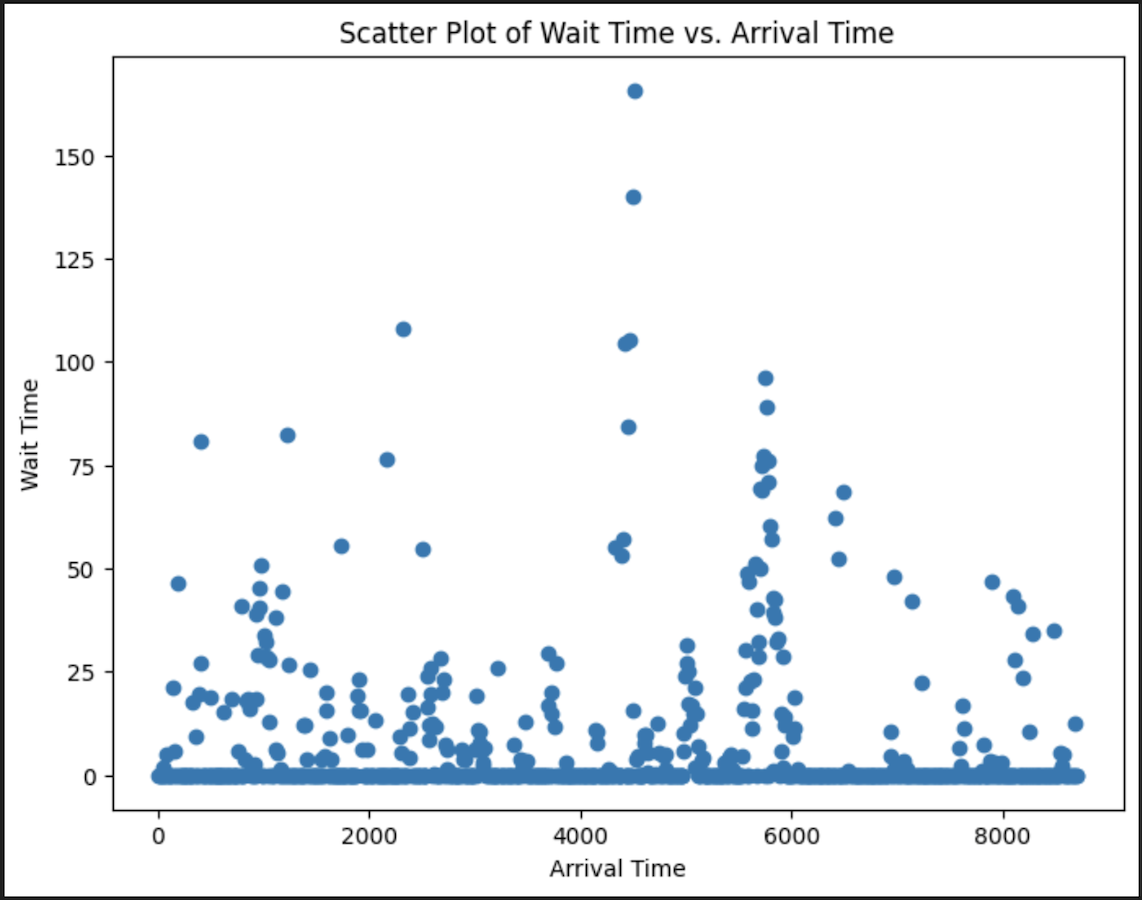
\includegraphics[width=\linewidth]{SIMULACION 1.png}  
        \caption{Wait Time vs Arrival Time}
        \label{fig:grafica2}
    \end{minipage}
    \end{figure}
        
    \subsection{Segunda Simulación}
    MINIMAL\_ARRIVAL\_TIME = 10 \\
    MAXIMUM\_ARRIVAL\_TIME = 20 \\
    
    En esta segunda simulación, hemos ajustado los tiempos de llegada de los barcos para que lleguen, en promedio, cada 15 horas. En comparación con la simulación anterior, el tiempo medio de espera es de casi 2 y solo 52 barcos de los 587 barcos anuales que pasan al año, tuvieron que esperar un tiempo considerable. Aunque hay una mejoría en comparación a la primera simulación; 10\% de espera todavía es alto y muestra que necesitamos ajustar más la programación de llegadas.

    \begin{figure}[H]
    \centering
    \begin{minipage}{0.5\textwidth}
        \centering
        \includegraphics[width=\linewidth]{SIMUlACION 2.1.png}  
        \caption{Number of boats per Type}
        \label{fig:grafica1}
    \end{minipage}\hfill
    \begin{minipage}{0.5\textwidth}
        \centering
        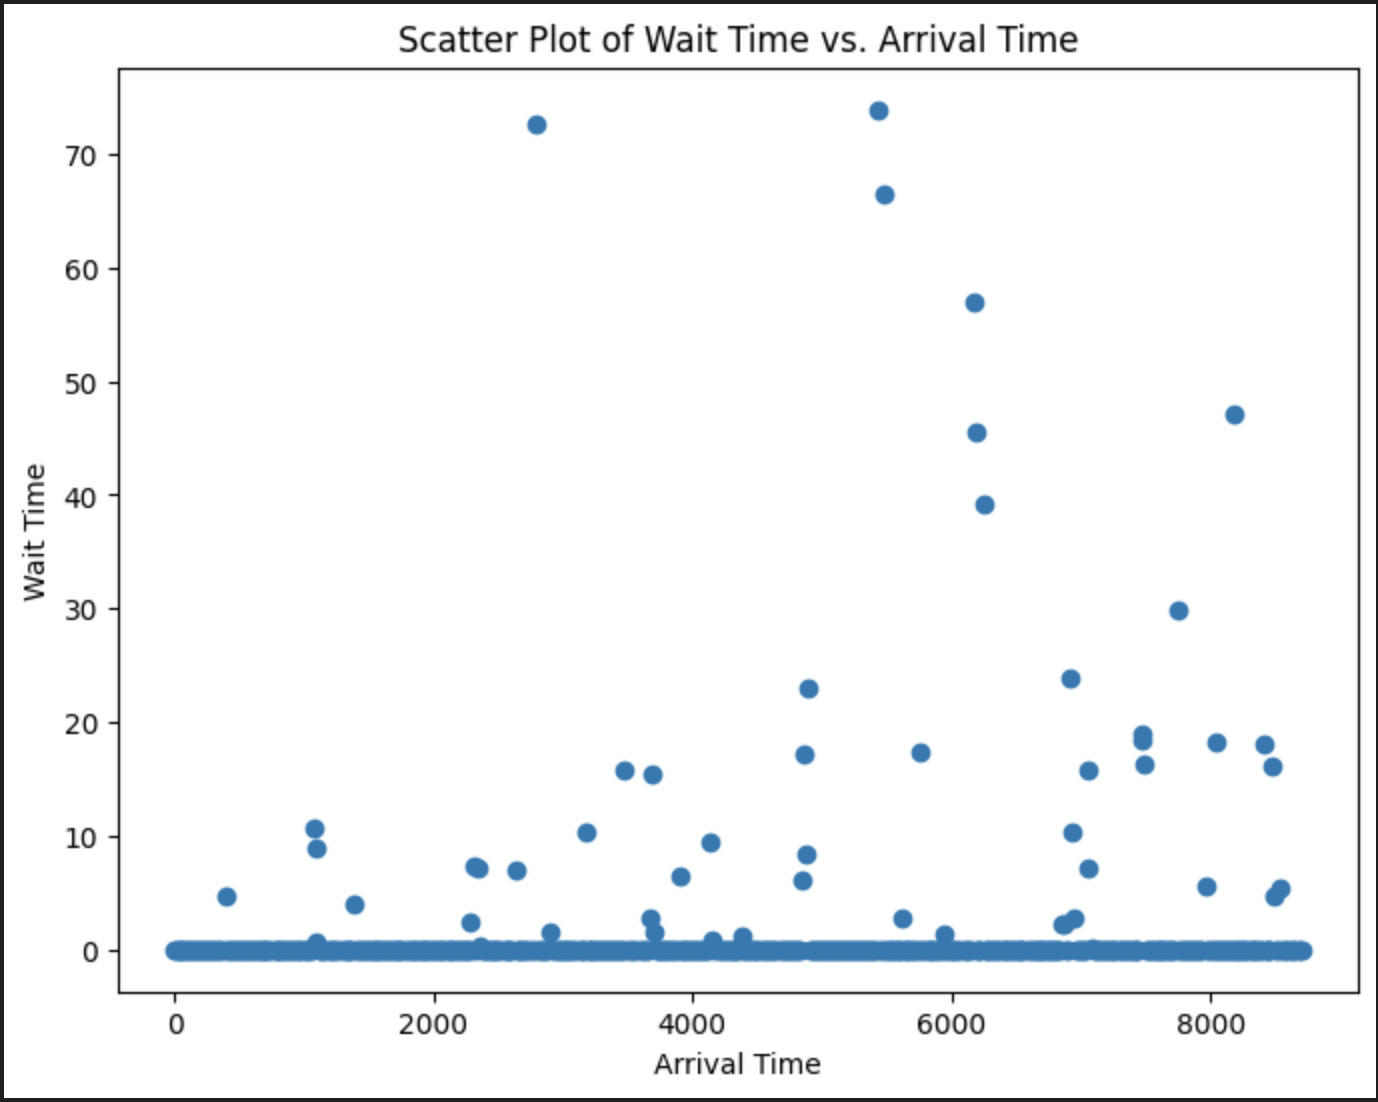
\includegraphics[width=\linewidth]{SIMULACION 2.png}  
        \caption{Wait Time vs Arrival Time}
        \label{fig:grafica2}
    \end{minipage}
    \end{figure}


    \subsection{Tercera Simulación}
    MINIMAL\_ARRIVAL\_TIME = 20 \\
    MAXIMUM\_ARRIVAL\_TIME = 30 \\

    En esta tercera y última simulación, con barcos llegando cada 25 horas (tiempos de espera de 20 a 30 horas), casi eliminamos las esperas. Se puede observar que solo 2 de los 346 barcos anuales enfrentaron demoras (dadas por imprevistos como problemas en el motor, inspección aleatoraia por aduanas o huelgas de trabajadores repentinas), lo cual es menos del 1\% (una mejora considerable en comparación con las anteriores simulaciones). Dicho suceso produjo unos a ingresos totales de 16 millones de euros y muestra que con una buena programación se puede operar el puerto de manera muy eficiente. Por lo tanto, es la simulación mas real

    \begin{figure}[H]
    \centering
    \begin{minipage}{0.5\textwidth}
        \centering
        \includegraphics[width=\linewidth]{SIMUlACION 3.1.png}  
        \caption{Number of boats per Type}
        \label{fig:grafica1}
    \end{minipage}\hfill
    \begin{minipage}{0.5\textwidth}
        \centering
        \includegraphics[width=\linewidth]{SIMUlACION 3.png}  
        \caption{Wait Time vs Arrival Time}
        \label{fig:grafica2}
    \end{minipage}
    \end{figure}

\end{document}
